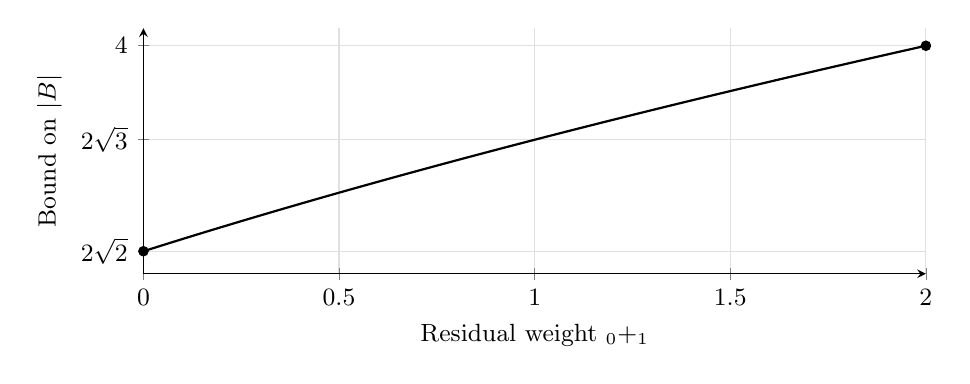
\begin{tikzpicture}
\begin{axis}[
 width=0.95\columnwidth,height=4.7cm,
 xmin=0,xmax=2,ymin=2.7,ymax=4.1,
 xlabel={Residual weight $\eps_0+\eps_1$},
 ylabel={Bound on $|B|$},
 xtick={0,0.5,1,1.5,2},
 ytick={2.82842712475,3.46410161514,4},
 yticklabels={$2\sqrt2$,$2\sqrt3$,$4$},
 tick label style={font=\small},label style={font=\small},
 axis lines=left,clip=false,grid=major,grid style={black!12},
 legend style={draw=none,font=\footnotesize}]
\addplot[black,thick,domain=0:2,samples=81] {sqrt(8+4*x)};
\addplot[only marks,mark=*,mark size=1.7pt,black] coordinates {(0,2.82842712475) (2,4)};
\end{axis}
\end{tikzpicture}
